N-Gram Graph (NGG) is a NPL tool initially proposed by George Giannakopoulos \cite{Ngram} that uses word or character n-grams in order to achieve documents summarization. The NGG tool basically slices the text in word or character n-grams and then represent them in a graph \emph{G = $\lbrace N,E,L,W\rbrace$} according to the following structure:
\begin{itemize}
	\item N is the set of nodes created for every different n-gram in the text
	\item E represent the edge of the graph; two nodes are connected if they are "close'' or within a \emph{distance window} from each other. The distance windows is denominated as neighbourhood distance
	\item L is a labelling function which assigns labels to every node and every edge (define the size of the n-gram)
	\item W is the weight function which assigns weights to every edge according to the number of times that two n-gram appear close one to the other
\end{itemize}

The big advantage coming from the use of this methodology is language
independence, since it makes no assumption on the underlying languages and
allows text manipulation trough graph operations.

In particular two operation are necessary for our goal:
\begin{itemize}
\item the \textbf{Merging or Union } operator, that given two graphs ($G_1$, $G_2$), returning a graph with all the edges, both common and uncommon, of the two operand graphs. The edges are weighted by the average of the weights of the original edges.
\item the \textbf{Intersection} operator between two graphs $G_1$ and $G_2$: which returns a graph with only the common edges of $G_1$ and $G_2$ averaging the weights of the original edges assigned as the new edge weights.
\item the \textbf{Normalized Value Similarity}[NVS] function that for every n-gram rank, indicating how many of the edges contained in graph $G_i$ are also contained in graph $G_j$, considering also the weights of the matching edges and normalize the result respect the graph size
\end{itemize}

In particular $NVS(G_i,G_j) = \frac{VS(G_i,G_j)}{SS(G_i,G_j)}$ where:
\begin{equation}
 VS(G_i,G_j)=\frac{\sum e \in G_i \frac{\min(w_e^i, w_e^j)}{\max(w_e^i, w_e^j)}}{\max(\mid G_i \mid, \mid G_j \mid)}
\end{equation}

\begin{equation}
 SS(G_i,G_j)=\frac{\min(\mid G_i \mid, \mid G_j \mid)}{\max(\mid G_i \mid, \mid G_j \mid)}
\end{equation}

Since NGG tools allow to compute both the tweet-news correlation and summary creation, this methodology is split in different section.

\subsubsection*{Tweet-News Correlation}
To compute the correlation between contradiction tweet and news, this methodology use the base idea of exploiting the NVS similarity function as a correlation function: higher the similarity between tweets graph representation and news graph, higher will be the correlation.

More in detail this procedure perform the following step:
\begin{itemize}
	\item compute the graph representation of the contradiction tweet (cTweetGraph[i])
	\item compute the  graph representation of the news inside the contradiction windows (insideNews[i])
\end{itemize}

Once we have the base component we use an algorithm to create a background knowledge about the topic.

\begin{algorithmic}
\FOR{New nw : allNews}
	\IF{ nw outside contradiction window }
		\STATE nGraph = DocumentNGramGraph(nw.getText());
		\STATE double NVS = Similarity(nGraph, insideNews[i]);
		\IF{NVS < similarityLimit}
			\STATE outsideNews[i].merge(newsGraph);
		\ENDIF
	\ENDIF
\ENDFOR
\STATE background[i] = insideNews[i].degrade(outsideNews[i]);
\end{algorithmic}

We have to compute the similarity between the outsideNews and the insideNews, since we want to filter form the outsideNews those article that are very similar respect to the insideNews.
We have to take this precaution because with a fixed timeWindows some news related to the main event can fall in the outsideNews.
This produce bad result when we create the background graph as the degraded version of the insideNews respect the outsideNews, since the degrade function decrease the weight of the common edges between insideNews and outsideNews.

When we have a good background we can compute the correlation for the news inside the contradiction window
\begin{algorithmic}
\FOR{News nw : allNews}
	\IF{nw inside contradiction window}
		\STATE nGraph = DocumentNGramGraph(nw.getText());
        \STATE nGraph = nGraph.intersectGraph(background[i]);
        \STATE NVS = Similarity(nGraph, cTweetGraph[i]);
	\ENDIF
\ENDFOR        
\end{algorithmic}

This approach requires a lot of computation, since have to compute the graph representation of the entire contradiction tweets set and of all news. Instead NGG allow to compute the similarity between text without the usage of grammar information and allow a controlled background removal function.

In figure \ref{fig:N-gram-expl} is possible to see how the algorithm work in a graphical way.


\begin{figure}[htbp]
	\centering
			{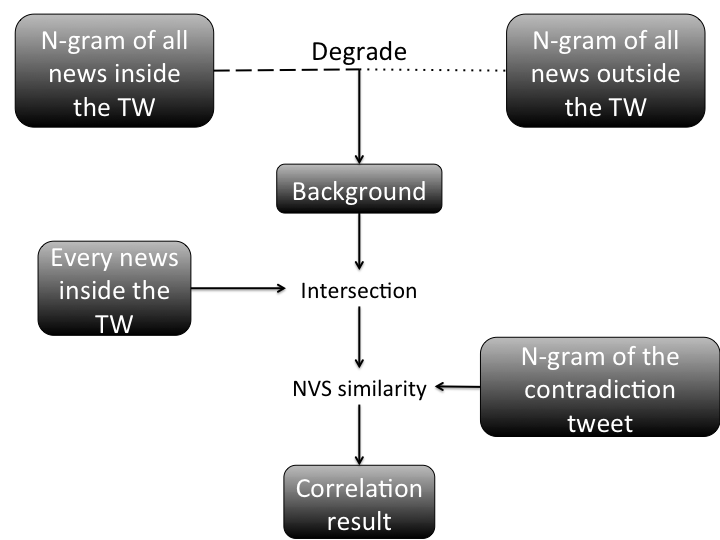
\includegraphics[width=8.5cm,height=7cm]{image/N-gram-expl.png}}	
		\caption[N-gram-expl]{Graphical explanation of how is computed the tweets-news correlation}
	\label{fig:N-gram-expl}
\end{figure} 

\subsubsection*{Summary Creation}
The second goal of this research is to create a summary of the event that cause the sentiment shift. 

For this purpose we use the news with the highest correlation value obtained at the step before.
Our choice was to limit the summary length to 150 word so there is no need to summarize many document. 


In particulate we select the candidate document to be summarized with the following procedure:


\begin{algorithmic}
\STATE stDev = standard deviation of the NVS values
\STATE sortNew[] = News sorted for decreasing NVS value
\FOR{i = 1 ; i < sortNew.length ; i++}
	\IF{ (i >=3) or (sortNew[i].getScore() <  (sortNew[0].getScore() - $stDev^2$))}
		\STATE sortNew.remove(i)
	\ENDIF
\ENDFOR
\end{algorithmic}


In this way we obtain at most three news to summarize and the intersection of the selected news will never be empty since we intersect quite similar news.

The summary algorithm perform the following action:


\begin{algorithmic}
\STATE newSentence[] = sentence of the candidate document
\FOR{ String sentence : newSentence }
	\STATE sGraph = DocumentNGramGraph(sentence);
    \STATE score.setValue(Similarity(sGraph, cTweetGraph[i]));
    \STATE score.setSentence(sentence)
    \STATE scoredSentence.add(score)
\ENDFOR
\STATE Arrays.sort(scoredSentence);
\end{algorithmic}

create the summary using the sentence with the highest NVS value until we reach 150 word.
This algorithm create a summary composed by the most significant sentences in news with the highest correlation value using a back-loop approach, but is not able to remove redundant sentences. Even so, a summary composed by sentences results to be more human readable than a list of key word.



